
\section{Results}

We ran several experiments to better characterize the properties of the randomized SOM and to compare them to the properties of a regular two-dimensional SOM. More specifically, we ran experiments using one dimensional, two dimensional and three dimensional datasets using uniform or shaped distributions. In this section, we only report a two-dimensional case and a three-dimensional case that we consider to be the most illustrative (all other results can be found in the supplementary material). We additionally ran an experiment using the MNIST hand-written data set and we compared it with a regular SOM. Finally, the last experiment is specific to the randomized SOM and shows how the model can recover from the removal (lesion) or the addition (neurogenesis) of neurons while conserving the overall self-organization. Each experiment (but the last) has been ran for both the randomized SOM and the regular SOM even though only the results for the randomized SOM are shown graphically in a dedicated figure while for the analysis, we use results from both SOM and RSOM. The reason to not show regular SOM results is that we assume the behavior is well known and does not need to be further detailed. 

\subsection{Two dimensional uniform dataset with holes}
\label{sec:2d-holes}

In order to test for the adaptability of the randomized SOM to different topologies, we created a two dimensional uniform dataset with holes of various size and at random positions (see figure \ref{fig:2D-holes:results}B). Such holes are known to pose difficulties to the regular SOM since neurons whose codewords are over a hole (or in the immediate vicinity) are attracted by neurons outside the holes from all sides. Those neurons hence become dead units that never win the competition. In the RSOM, this problem exists but is less severe thanks to the absence of regularity in the underlying neural topology and the loose constraints (we use 2 neighbors to build the topology). This can be observed in \ref{fig:2D-holes:results}B) where the number of dead units is rather small and some holes are totally devoid of any neurons. Furthermore, when a sample that does not belong to the original distribution is presented, it can be observed that the answer of the map is maximal for a few neurons only (see figure \ref{fig:2D-holes:results}G)).


%The second experiment is designed to investigate how the SOM algorithms cope with two-dimensional uniformly distributed data points with holes ($x_1, x_2 \sim \mathcal{U}(0, 1)$). Therefore, in this case the input to the maps is two-dimensional Euclidean points on a plane, where we put some holes at random places on the plane (see Figure~\ref{Fig:persistence_exp2b} {\bfseries \sffamily B}, blue discs). We train again both the VSOM and the Kohonen maps over $25000$ samples for $25000$ epochs and each map consists of $1024$ neurons. For the VSOM we define the topology of the map using a blue noise distribution (see Figure~\ref{Fig:experiment2b} {\bfseries \sffamily A}) and for the Kohonen we use the standard rectangular Euclidean grid. After convergence both algorithms generate proper topographic maps covering the  input space. Figure~\ref{Fig:experiment2b} {\bfseries \sffamily B} shows the mapping of VSOM learning algorithm (white discs and black segments) along with the input space (blue discs). We observe that not too many neurons cover the holes.

This observation is also supported by our topological analysis shown in figure \ref{fig:2D-holes:analysis}. Figures
\ref{fig:2D-holes:analysis}A, B, and C show the persistent barcodes where we can see the lifespan of each (birth, death)
pair (for more details about how we compute these diagrams see Section~\ref{sec:tda}). We observe that both the SOM and
the RSOM capture both the $H0$- and $H1$-homology of the input space, however the RSOM seems to have more persistent 
topological features for the $H1$-homology (orange lines). This means that the RSOM can capture more accurately the 
holes which are present in the input space. Roughly speaking we have about eight holes (see figure~\ref{fig:2D-holes:results}B) and we count about eight persistent features (the longest line segments
in the barcode diagrams) for RSOM in \ref{fig:2D-holes:analysis}C. On the other hand, the important persistent features
for the SOM are about five. In a similar way the persistent diagrams in figures~\ref{fig:2D-holes:analysis}C, D, and E
show that both RSOM and SOM capture in a similar way both the $H0$- and $H1$-homology features, although the 
RSOM (panel F) captures more holes as the isolated orange points away from the diagonal line indicate. This
is because the pairs that are further away from the diagonal are the most important meaning that they represent 
topological features that are the most persistent during the filtration process. 
Furthermore, we measure the Bottleneck distance between the persistence diagrams of input space and those of 
SOM and RSOM. The SOM's persistence diagram for $H0$ is closer to the input space (SOM: $0.000829$, RSOM: $0.001$),
while the RSOM's persistence diagram is closer to input's one for the $H1$ (SOM: $0.00478$, RSOM: $0.0037$). 
Finally, we ought to point out that the scale between panels A (D) and B, C (E, F) are not the same since the 
self-organization process has compressed information during mapping the input space to neural one.


% On the upper part of this figure, we can see that the 1-homology (or H1, blue segments, blue dots) are more elongated for RSOM (last column) when compared to the regular SOM (central column). These segments correspond to the lifespan of H1 features when the $\alpha$ radius is increased and we can observe that the RSOM is closer to the actual distribution (left column) when compared to SOM. More precisely, we observe that the number of holes in figure~\ref{fig:2D-holes:results} is eight. Furthermore, we notice that the number of persistent blue segments (first raw of figure~\ref{fig:2D-holes:analysis}) in persistent barcodes of figure~\ref{fig:2D-holes:analysis} is about eight for the input space and about the same for the RSOM. The regular SOM expresses less persistent blue segments. The length of the blue or red segments in the barcodes indicate the lifespan  of the filtration under the variation of radius $\alpha$. The more a segment survives the more important that topological feature is. Therefore, we can claim that the RSOM has about six persistent (significant) blue segments meaning that there are eight \emph{holes} in the corresponding neural space. On the contrary, regular SOM has less persistent segments of 1-homology (blue lines) implying that it covers more regularly the input space. Similar results are shown in the second raw of figure~\ref{fig:2D-holes:analysis}, where the persistent diagrams display the pairs (birth, death). Every time the radius $\alpha$ increases new pairs are born or die as we have already described in Section~\ref{sec:topo}. 


% However, 0-homology (H0, red segments) of RSOM and SOM behavior is very similar but also quite different from the actual distribution. 

% \npr{ Here, an explanation of what are the red lines would be necessary. Also, concerning H0, I'm not sure how to explain the difference with SOM, RSOM and the actual distribution and what does that mean.}

%Differences in $H0$ are attributed to the different neural space topology the two algorithms, the Kohonen and the VSOM, use. VSOM's neurons are placed not on an rectangular Euclidean grid as Kohonen's do, but instead on a random (following a blue noise distribution) Euclidean grid. 

% \npr{ Where is the referenced figure below? Where is the explanation concerning birht death rate on the analysis figure ?}


% In Figures~\ref{Fig:experiment2b} {\bfseries \sffamily C}-{\bfseries \sffamily H} we show the receptive fields of six randomly chosen units from the VSOM  map. We see that different stimuli are captured by different units implying that the topographic map of VSOM map is well-formed. 



\begin{figure}
  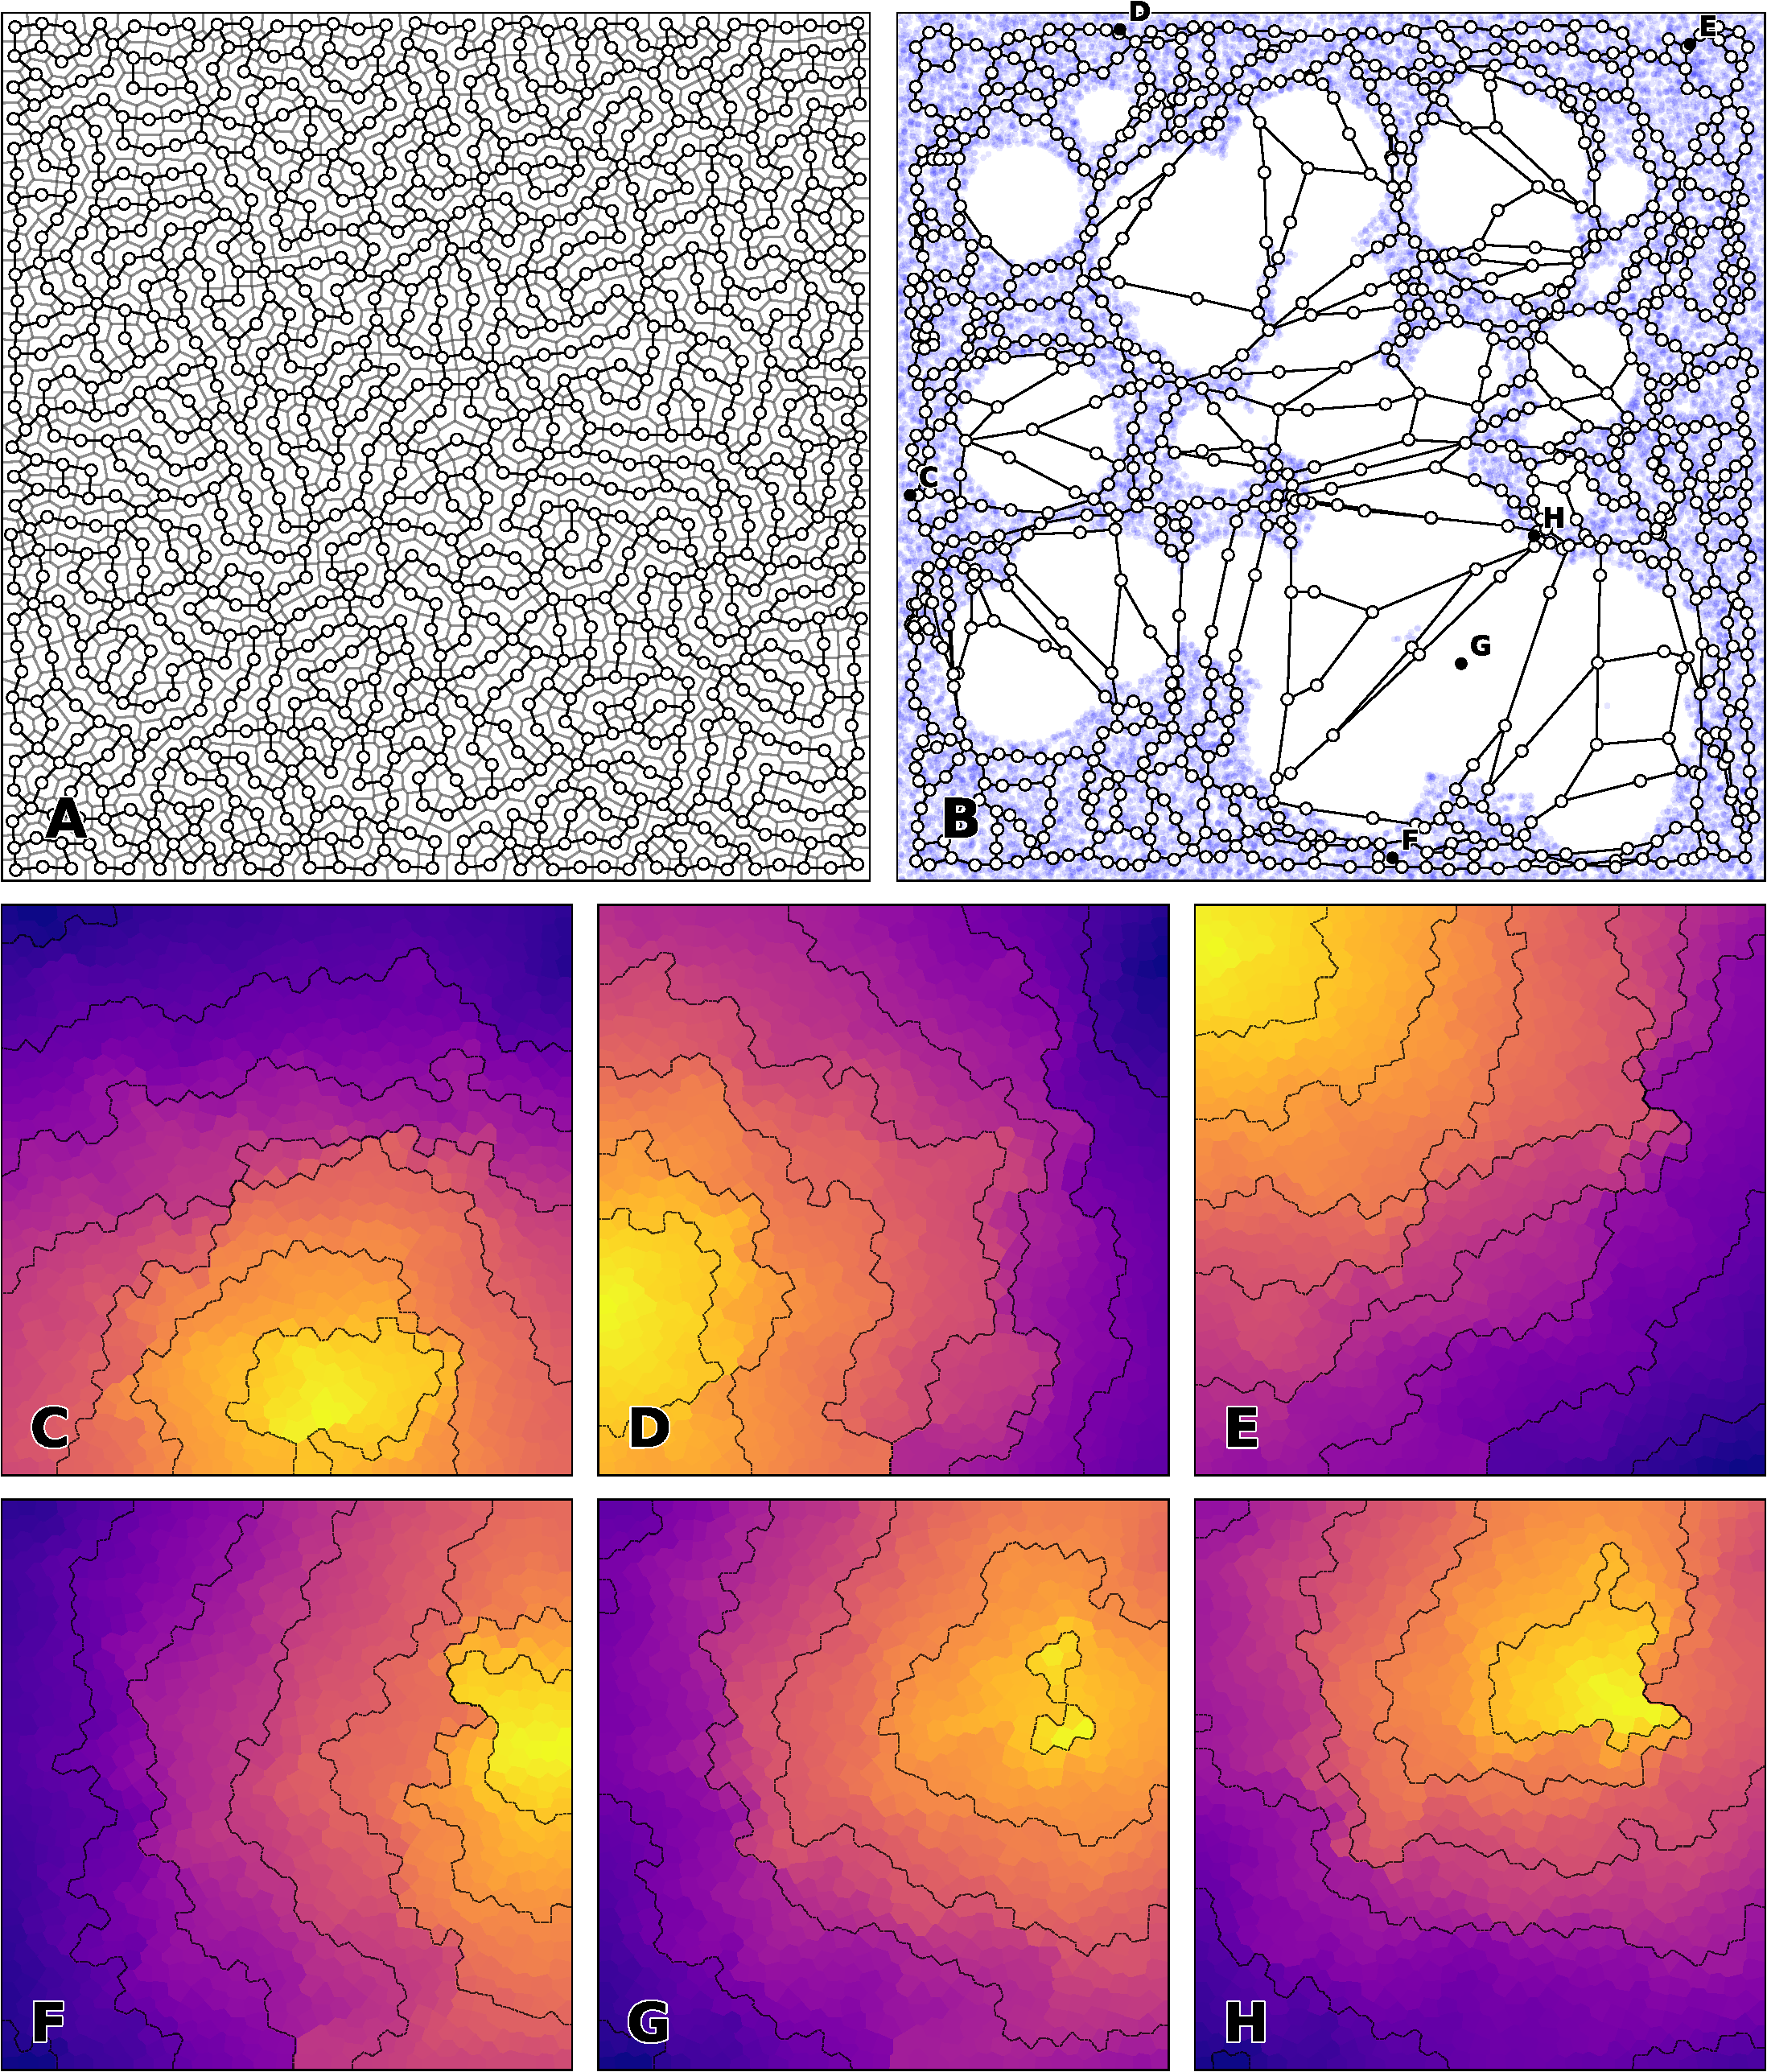
\includegraphics[width=\columnwidth]{experiment-2D-holes.pdf}
  \vspace{2mm}
  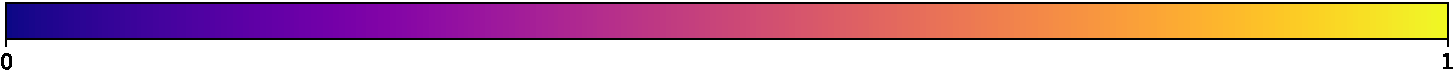
\includegraphics[width=\columnwidth]{figures/colormap.pdf}
  %
  \caption{%
  %
  {\bfseries \sffamily Two dimensional uniform dataset with holes (results)}
  %
  Randomized SOM made of $1024$ neurons with a $2$-nearest neighbors induced topology. Model has been trained for $25,000$ epochs on two-dimensional points drawn from a uniform distribution on the unit square with holes of various sizes and random positions. \textbf{A} Map topology in neural space. \textbf{B} Map topology in data space. \textbf{C to H} Normalized distance map for six random samples. The \textbf{G} point has been purposely set outside the point distribution. Normalization has been performed for each sample in order to enhance contrast but this prevents comparison between maps.
  %
  }
  \label{fig:2D-holes:results}
\end{figure}

\begin{figure}
  \centering
  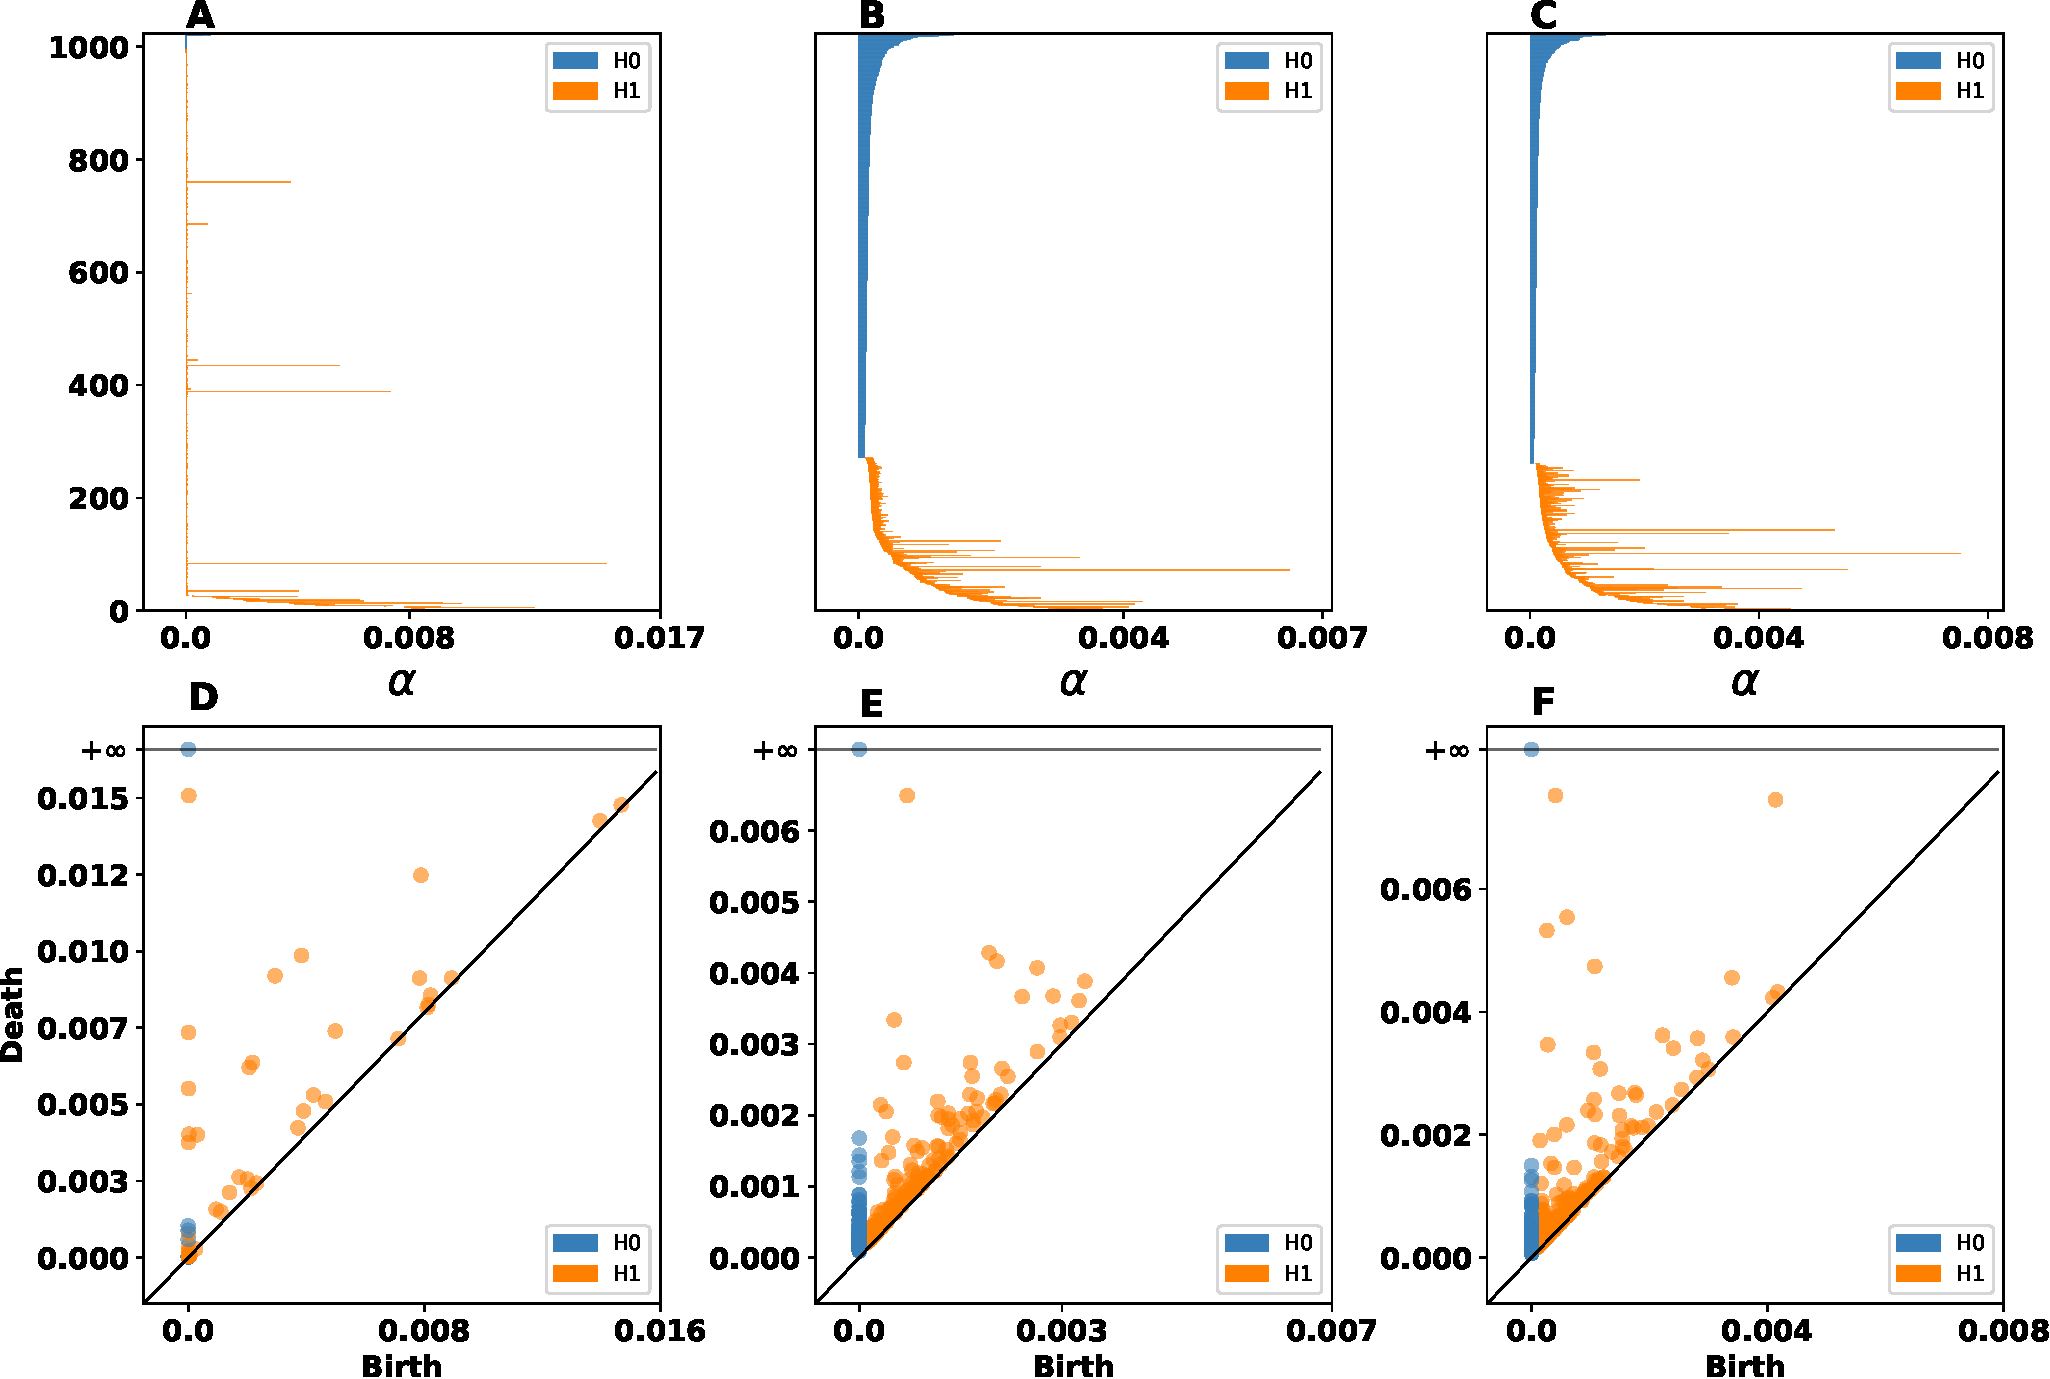
\includegraphics[width=\columnwidth]{experiment-2D-holes-analysis.pdf}
  %
  \caption{{\bfseries \sffamily Two dimensional uniform dataset with holes (analysis)}
  Persistent Barcodes of \textbf{A} input space, \textbf{B} SOM, and \textbf{RSOM}.
  The blue and orange line segments represent the $H0$- and $H1$-homology, respectively. This means
  that blue color represents connected segments within the space and orange color reflects the holes
  within the space. The longer the line segment the more important the corresponding topological
  feature. \textbf{D} illustrates the persistent diagram for the input space. \textbf{E} and \textbf{F}
  depict the persistent diagrams for SOM and RSOM, respectively. Again blue dots indicate $H0$-homology
  features and orange dots represent $H1$-homological features.}
  \label{fig:2D-holes:analysis}
\end{figure}

\subsection{Three dimensional uniform dataset}

The three dimensional uniform dataset (that corresponds to the RGB color cube) is an interesting low dimensional case that requires a dimensionality reduction (from dimension 3 to 2). Since we used a uniform distribution this means the dataset is a dense three dimensional manifold that needs to be mapped to a two dimensional manifold which is known not to have an optimal solution. However, this difficulty can be partially alleviated using a loose topology in the RSOM. This is made possible by using a 2-neighbours induced topology as shown in figure \ref{fig:3D-uniform:results}A. This weak topology possesses several disconnected subgraphs that relax the constraints on the neighborhood of the BMU (see figure \ref{fig:topology-influence} in the supplementary section for the influence of neighborhood on the self-organization). This is clearly illustrated in figure \ref{fig:3D-uniform:results}B where the Voronoi cell of a neuron has been painted with the color of its codeword. We can observe an apparent structure of the RGB spectrum with some localized ruptures. To test for the completeness of the representation, we represented the position of six fundamental colors (C - white (1,1,1), D - black (0,0,0), E - yellow (1,1,0), F - red (1,0,0), G - green (0,1,0) and H - blue (0,0,1)) along with their associated distance maps after learning.

Furthermore, we performed the persistent homology to identify important topological features in the
input space and investigate how well the SOM and RSOM captured those features. Figures
\ref{fig:3D-uniform:analysis}A, B, and C show the persistent barcodes for the input space, SOM, and 
RSOM, respectively. We can see how the RSOM (panel C) captures more $H1$- and $H2$-homological properties
(since there are more persistent line segments, orange and green lines). The SOM (panel B) seems to capture
some of those features as well but they do not persist as long as they in the case of RSOM. The persistence 
diagrams of input, SOM and RSOM are shown in figures~\ref{fig:3D-uniform:analysis} D, E, and F, respectively.
These figures indicate that the RSOM has more persistent features (orange and green dots away from the diagonal
line) than the regular SOM.
The Bottleneck distance between the persistence diagrams of input space and those of SOM and RSOM reveals
that the SOM's persistence diagram is slightly closer to the input space's one for both the $H0$ (SOM: $0.00035$,
RSOM: $0.0007$), $H1$ (SOM: $0.006$, RSOM: $0.007$), and $H2$ (SOM: $0.0062$, RSOM: $0.0057$). Despite the 
fact that the bottleneck distances show that 
regular SOM's persistent diagram is closer to input space's one, the barcodes diagrams indicate that the RSOM 
captures more persistent topological features suggesting that RSOM preserves in a better way the topology of the
input space. Furthermore, the RSOM seems to capture better the higher dimensional topological features since the 
Bottleneck distances of $H2$-homological features are smaller for the RSOM than for the SOM.

% For the three-dimensional experiment we draw 50,000 three-dimensional points from a uniform distribution $\mathcal{U}([0, 1]\times [0, 1]\times [0, 1])$ (the cloud points form a cube in $\mathbb{R}^3$). The map is a two-dimensional manifold and thus the required task it to map the three-dimensional vectors  to the two-dimensional neural space. Once again we place the neurons on the two-dimensional neural space based on the sampling of a blue noise distribution and the induced topology is illustrated in Figure~\ref{fig:3D-uniform:results}A. The learning algorithm runs for $25000$ epochs over the three-dimensional vectors and after convergence we  obtain the map with the prototypes shown in Figure~\ref{fig:3D-uniform:results}B. Each color represents a different face of the three-dimensional cube (a cube has six faces so we obtain mainly six colors) and we observe that the SOM has mapped the three-dimensional cube on a two-dimensional neural space. The continuity and grouping of the colors indicates that the receptive fields of the neurons have been established properly. We illustrate this phenomenon in panels~\ref{fig:3D-uniform:results}C-H,  where the response of six different neurons (see the annotation in panel~\ref{fig:3D-uniform:results}B). The dark blue color indicates values close to zero and the yellow color represents values close to one.


\begin{figure}
  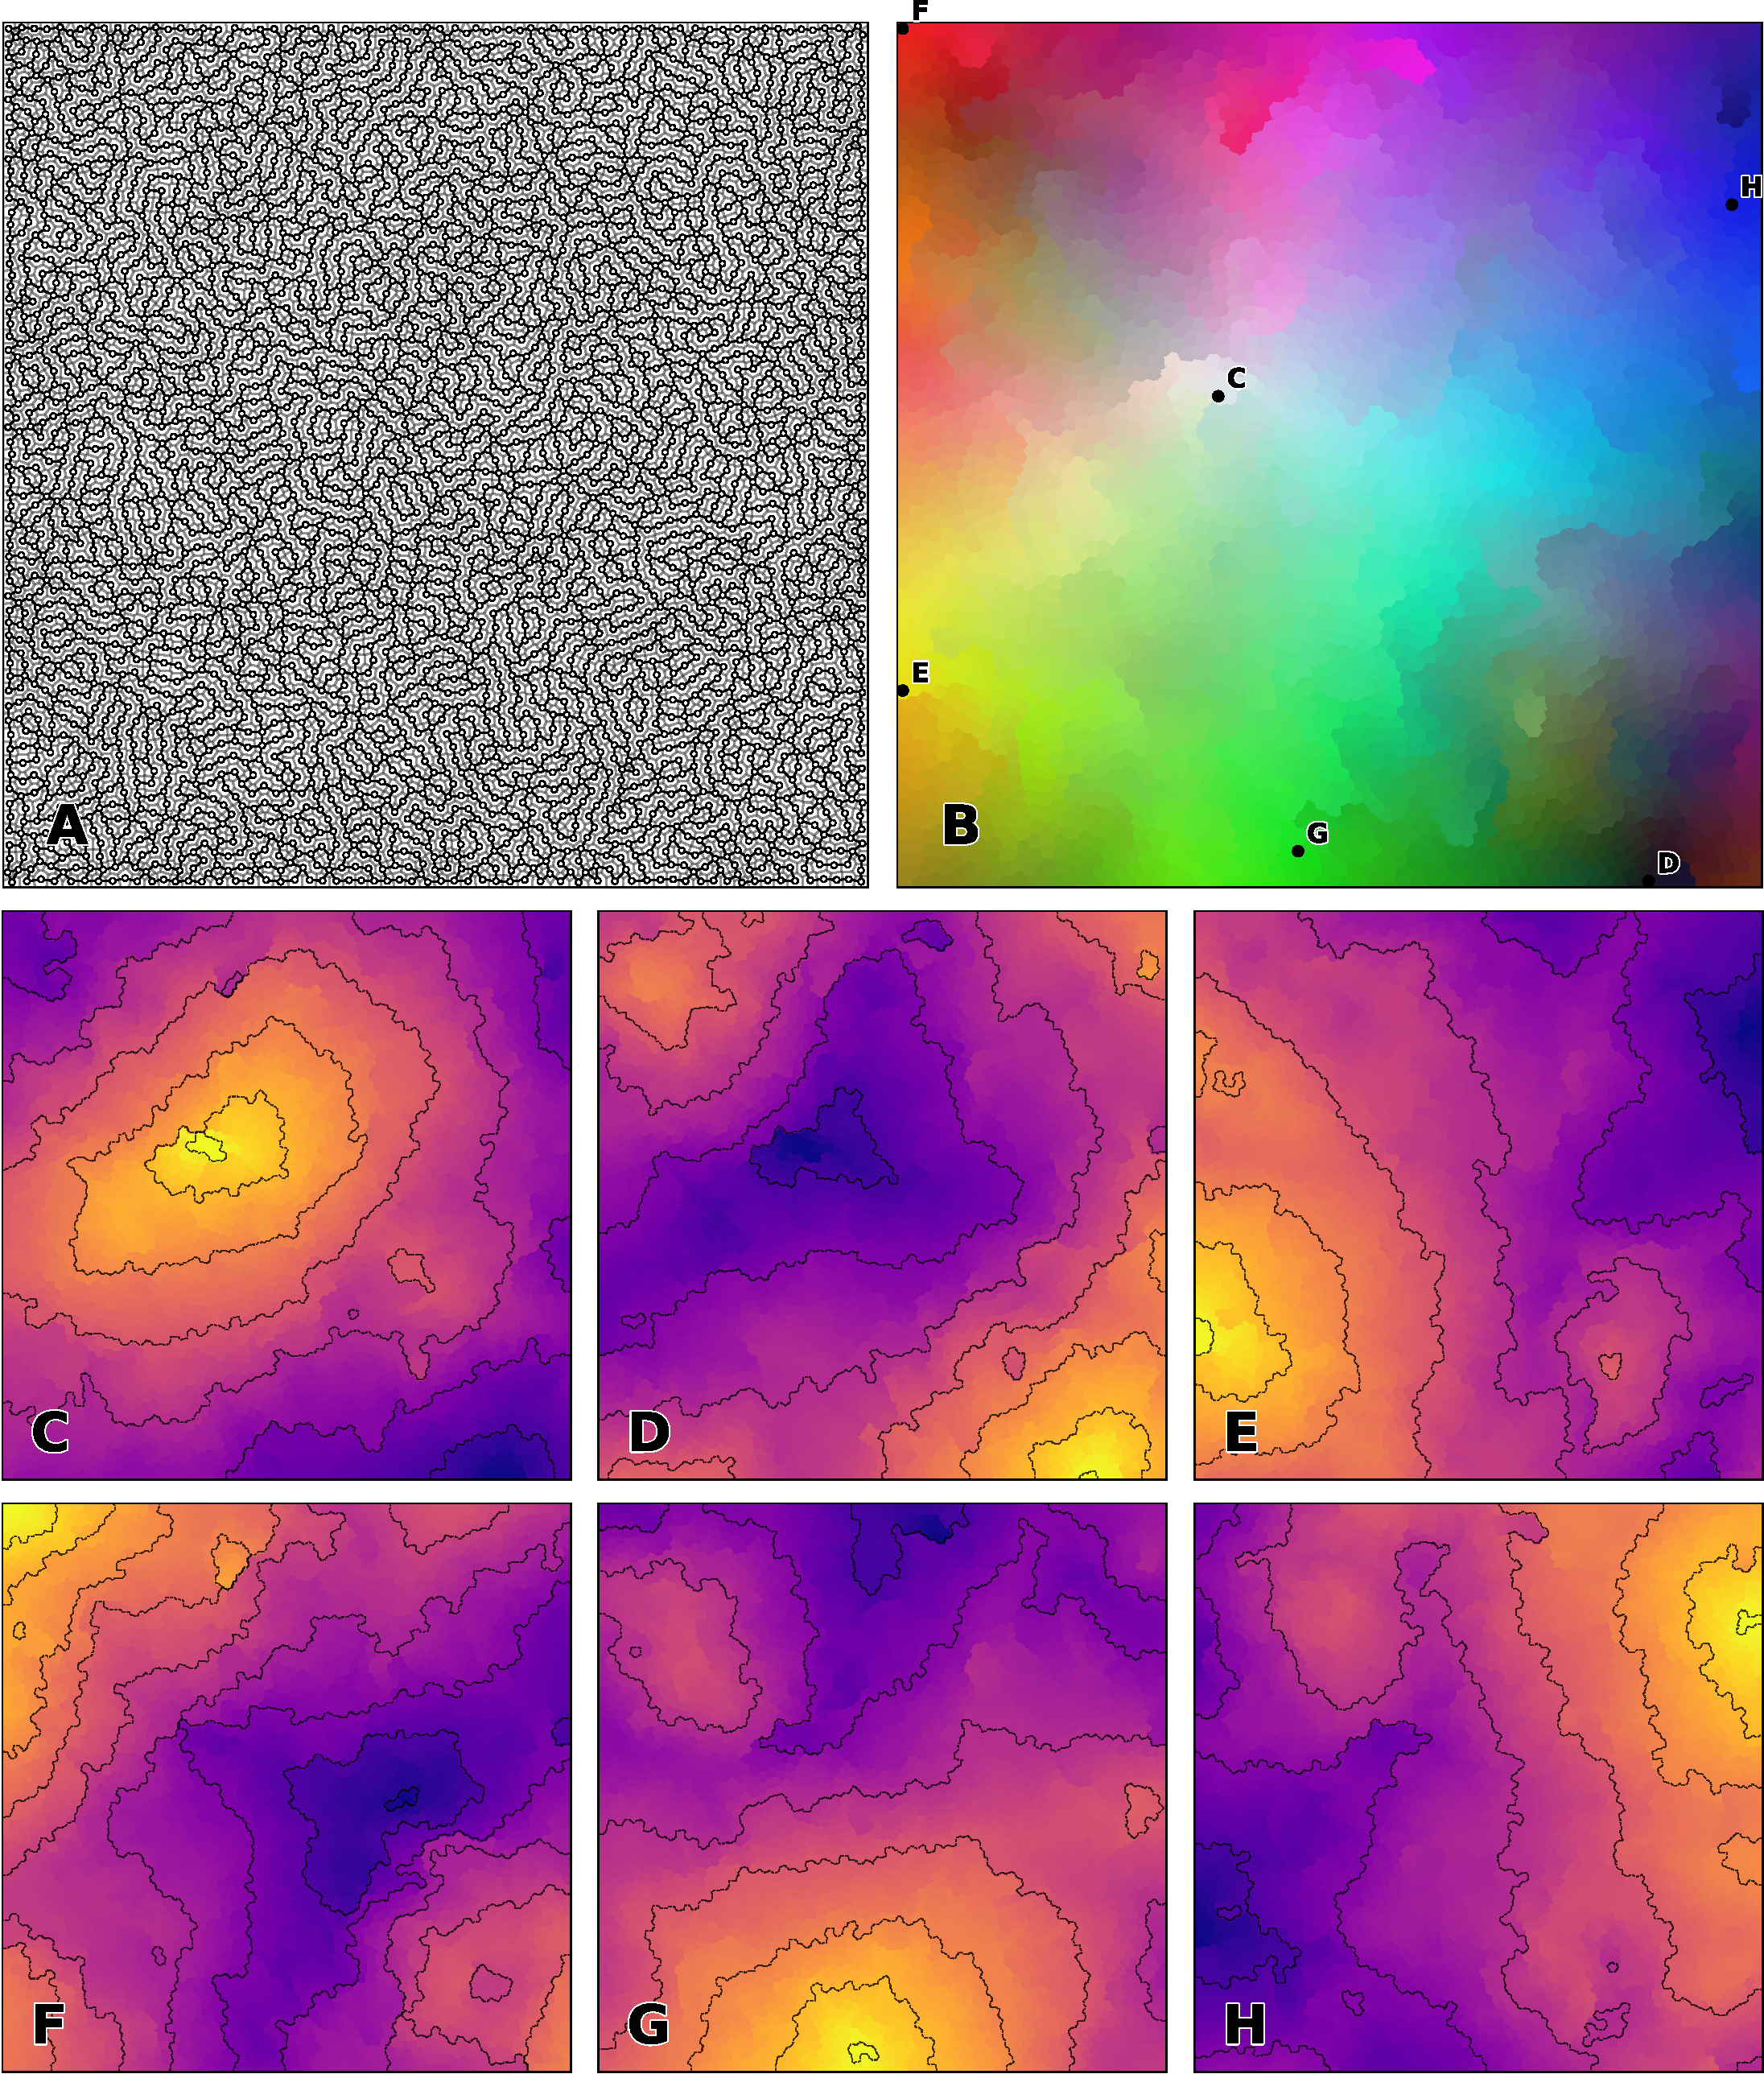
\includegraphics[width=\columnwidth]{experiment-3D-uniform.pdf}
  \vspace{2mm}
  \centering
  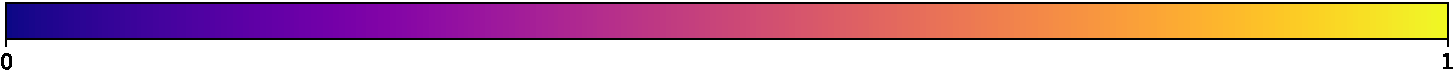
\includegraphics[width=.975\columnwidth]{figures/colormap.pdf}
  %
  \caption{%
  %
  {\bfseries \sffamily Three dimensional uniform dataset (results)}
  %
  Randomized SOM made of $4096$ neurons with a $3$-nearest neighbors induced topology. Model has been trained for $25,000$ epochs on three-dimensional points drawn from a uniform distribution on the unit cube. \textbf{A} Map topology in neural space. \textbf{B} Map codeword in neural space. Each neural voronoi cell is painted with the color of the codeword. \textbf{C to H} Normalized distance map for six samples, respectively (1,1,1), (0,0,0), (1,1,0), (1,0,0), (0,1,0) and (0,0,1) in RGB notations. Normalization has been performed for each sample in order to enhance contrast but this prevents comparison between maps.
  %
  }
  \label{fig:3D-uniform:results}
\end{figure}

\begin{figure}
     \centering
     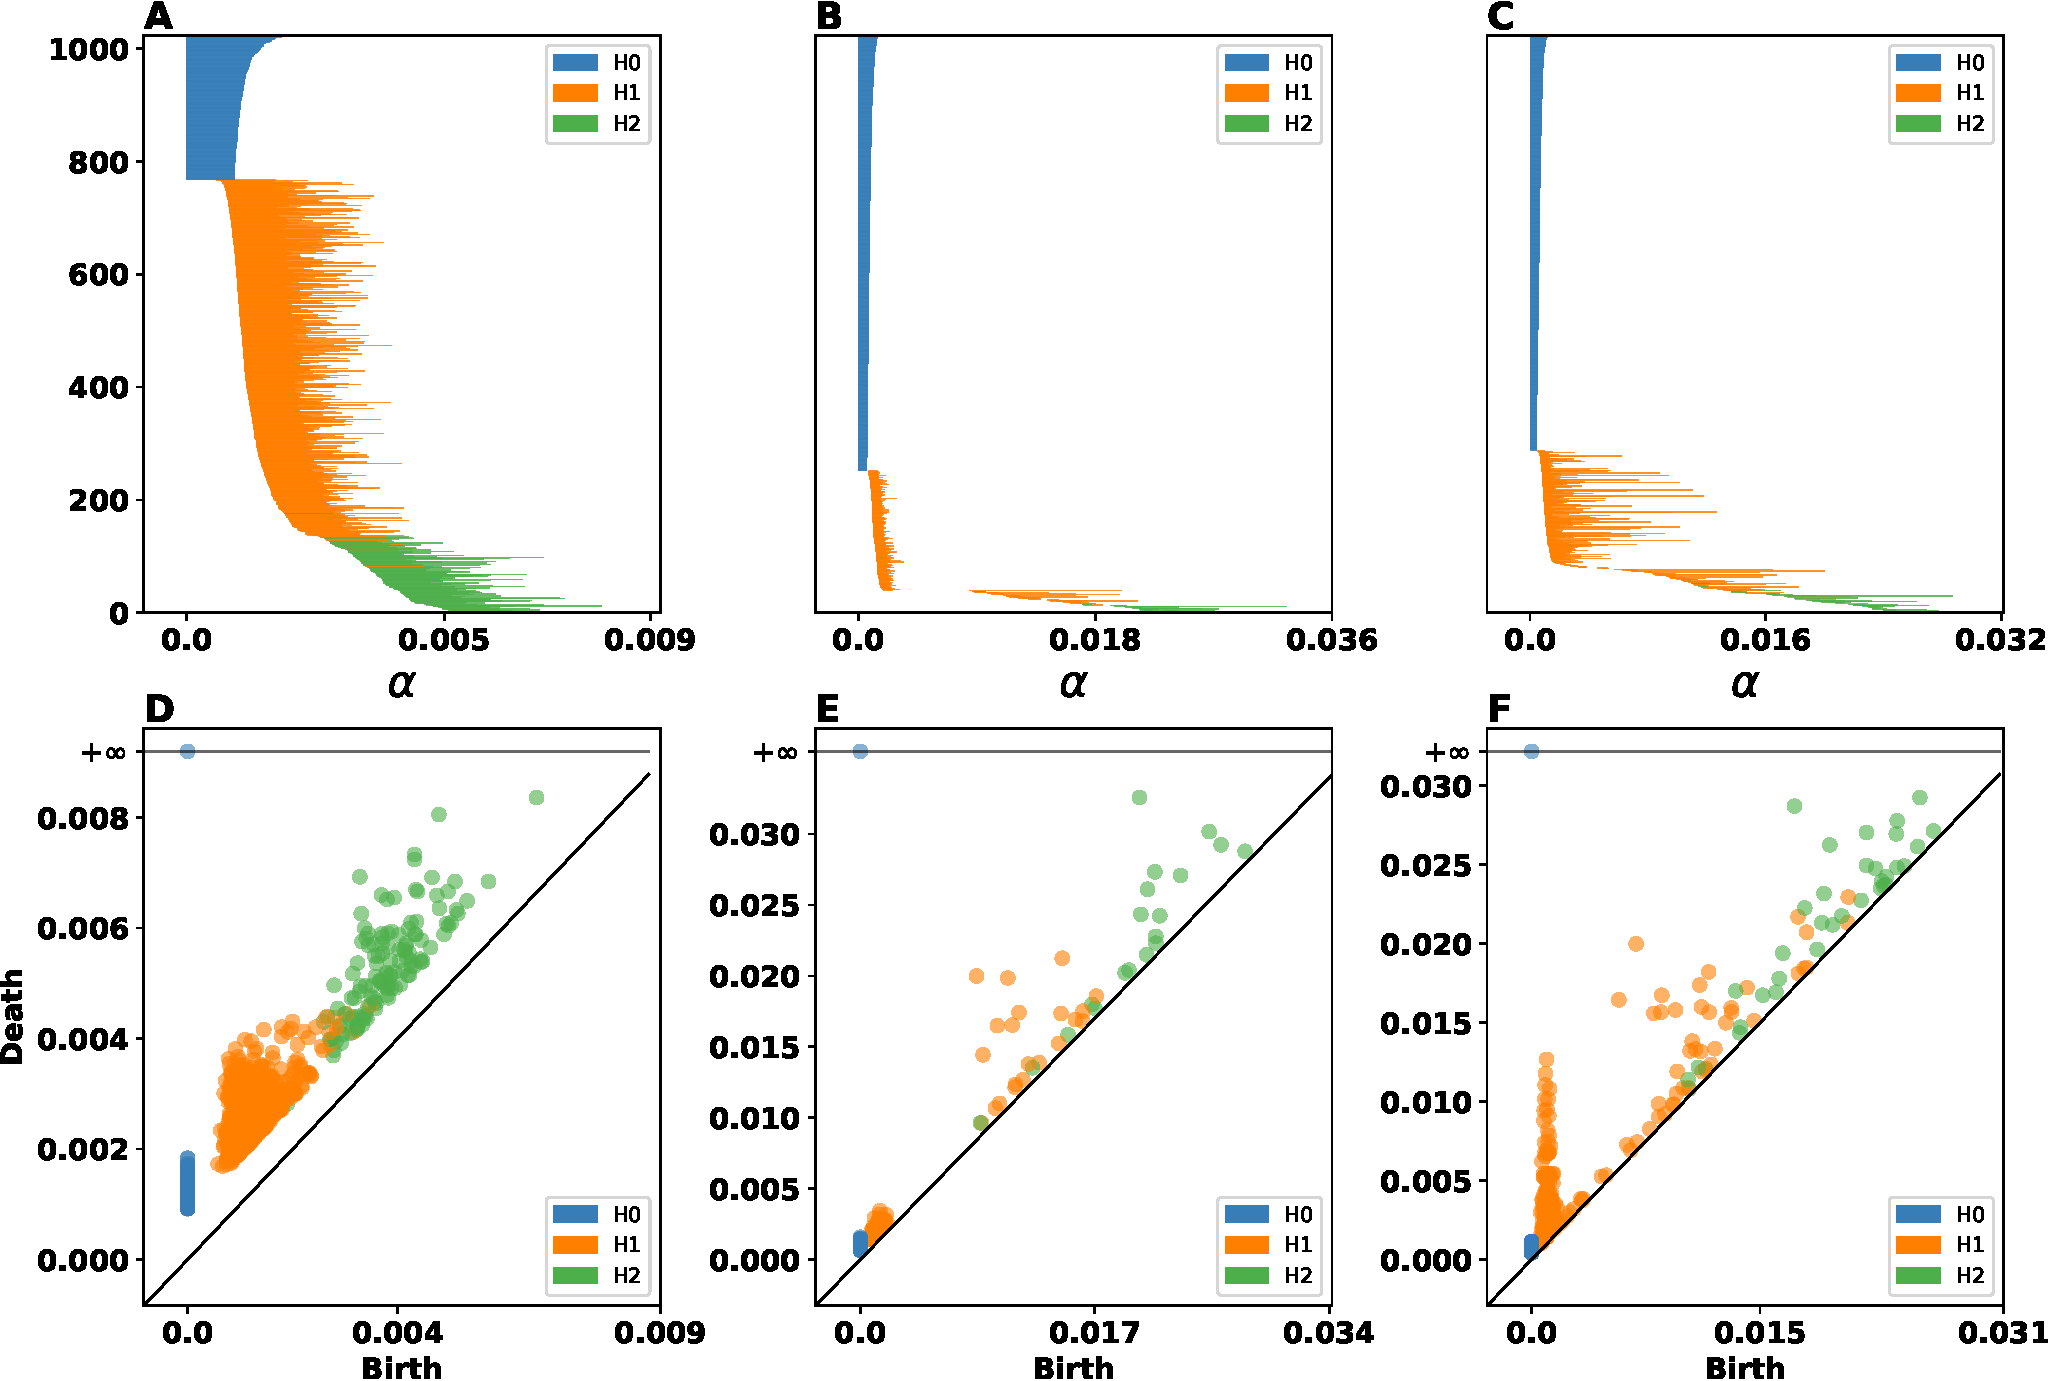
\includegraphics[width=\textwidth]{figures/experiment-3D-uniform-analysis.pdf}
     \caption{ {\bfseries \sffamily Three dimensional uniform dataset (analysis)}
     Persistent Barcodes of \textbf{A} input space, \textbf{B} SOM, and \textbf{RSOM}.
  The blue, orange, and green line segments represent the $H0$-, $H1$-, and $H2$-homology, respectively.
  This means that blue color represents connected segments within the space and orange color reflects the holes
  within the space and the green one the voids. The longer the line segment the more important the 
  corresponding topological feature. \textbf{D} illustrates the persistent diagram for the input space.
  \textbf{E} and \textbf{F} depict the persistent diagrams for SOM and RSOM, respectively. Again blue dots
  indicate $H0$-homology features, orange dots represent $H1$-homolocical features, and green the 
  $H2$-homological features.}
 \label{fig:3D-uniform:analysis}
\end{figure}


\subsection{MNIST dataset}

We tested RSOM on the standard MNIST dataset \citep{Lecun:1998} that contains $60,000$ training images and $10,000$ testing images. The dimension of each image is 28$\times$28 pixels and they are encoded using grayscale levels as the result of the normalization of the original black and white NIST database. The standard performance on most algorithms on the MNIST dataset is below 1\% error rate (with or without preprocessing) while for the regular SOM it is around 90\% recognition rate depending on the initial size, learning rate, and neighborhood function. Our goal here is not to find the best set of hyper-parameters but rather to explore if SOM and RSOM are comparable for a given set of hyper-parameters. Consequently, we considered a size of 32$\times$32 neurons and used the entire training set (60,000 examples) for learning and we measured performance on the entire testing set. We did not use any preprocessing stage on the image and we fed directly each image of the training set with the associated label to the model. Labels (from 0 to 9) have been transformed to a binary vector of size 10 using one-hot encoding (e.g. label 3 has been transformed to 0000001000). These binary labels can then be learned using the same procedure as for the actual sample. To decode the label associated to a code word, we simply consider the argmax of these binary vectors. Figure \ref{fig:MNIST:results} shows the final self-organisation of the RSOM where the class for each cell has been colorized using random colors. We can observe a number of large clusters of cells representing the same class (0, 1, 2, 3, 6) while the other classes (4,5,7,8,9) are split in two or three clusters. Interestingly enough, the codewords at the borders between two clusters are very similar. In term of recognition, this specific RSOM has an error rate just below 10\% ($0.903,\, \pm 0.296$) which is quite equivalent to the regular SOM error rate ($0.906,\, \pm 0.292$). The perfomances of the RSOM and SOM are actually not significantly different, suggesting that the regular grid hypothesis can be weaken.

In a similar way we measured the similarity of the neural spaces generated by both the regular SOM and the RSOM using the persistent diagram and barcodes. The only significant difference from previous analysis was the projection of the input and neural spaces to a lower-dimension space via UMAP \citep{Mcinnes:2018}. Projections of high-dimensional spaces to lower-dimension ones have been used before in the analysis of latent spaces of autoencoders \citep{Detorakis:2019}. Here, we use the UMAP since it's an efficient and robust method for applying a dimensionality reduction on input and neural spaces. More precisely, we project the MNIST digits as well as the code words (dimension $784$) to a space of dimension $7$. Once we get the projections, we proceed to the topological analysis using the persistent diagram and barcodes as we already have described in previous paragraphs.
Figure~\ref{fig:MNIST:analysis} shows the results regarding the persistent barcodes and diagrams. 
The persistent barcodes in figures~\ref{fig:MNIST:analysis}A, B, and C indicate that RSOM captures more 
persistent features (panel C, orange and green lines reflect the $H1$- and $H2$-homological features, respectively)
than the regular SOM (panel B). The persistence diagrams of input, SOM and RSOM are shown in 
figures~\ref{fig:MNIST:analysis} D, E, and F, respectively. 
These figures indicate that the RSOM has more persistent features (orange and green dots away from the diagonal
line) than the regular SOM, consistently with the two previous experiments ($2$D uniform distribution with holes
and $3$D uniform distribution). The Bottleneck distance between the persistence diagrams of input space and 
those of SOM and RSOM for the $H0$ are SOM: $1.0$ and RSOM: $1.12$, for $H1$ SOM: $0.19$ and RSOM: $0.22$, and
finally for the $H2$ are SOM: $0.05$ and RSOM:$0.05$. Again we observe that the regular SOM has a persistent 
diagram that is closer to the one of the input space than that of RSOM, however the RSOM seems to approache 
slightly better the input space topology since it has more pairs (birth, death) away from the diagonal (black
line) in figures~\ref{fig:MNIST:analysis}D, E, and F. Moreover, the persistent barcode of RSOM (figure~\ref{fig:MNIST:analysis}C indicates that has more persistent features for the radius $\alpha$
between $0$ and $1.512$ than the regular SOM.

\begin{figure}
  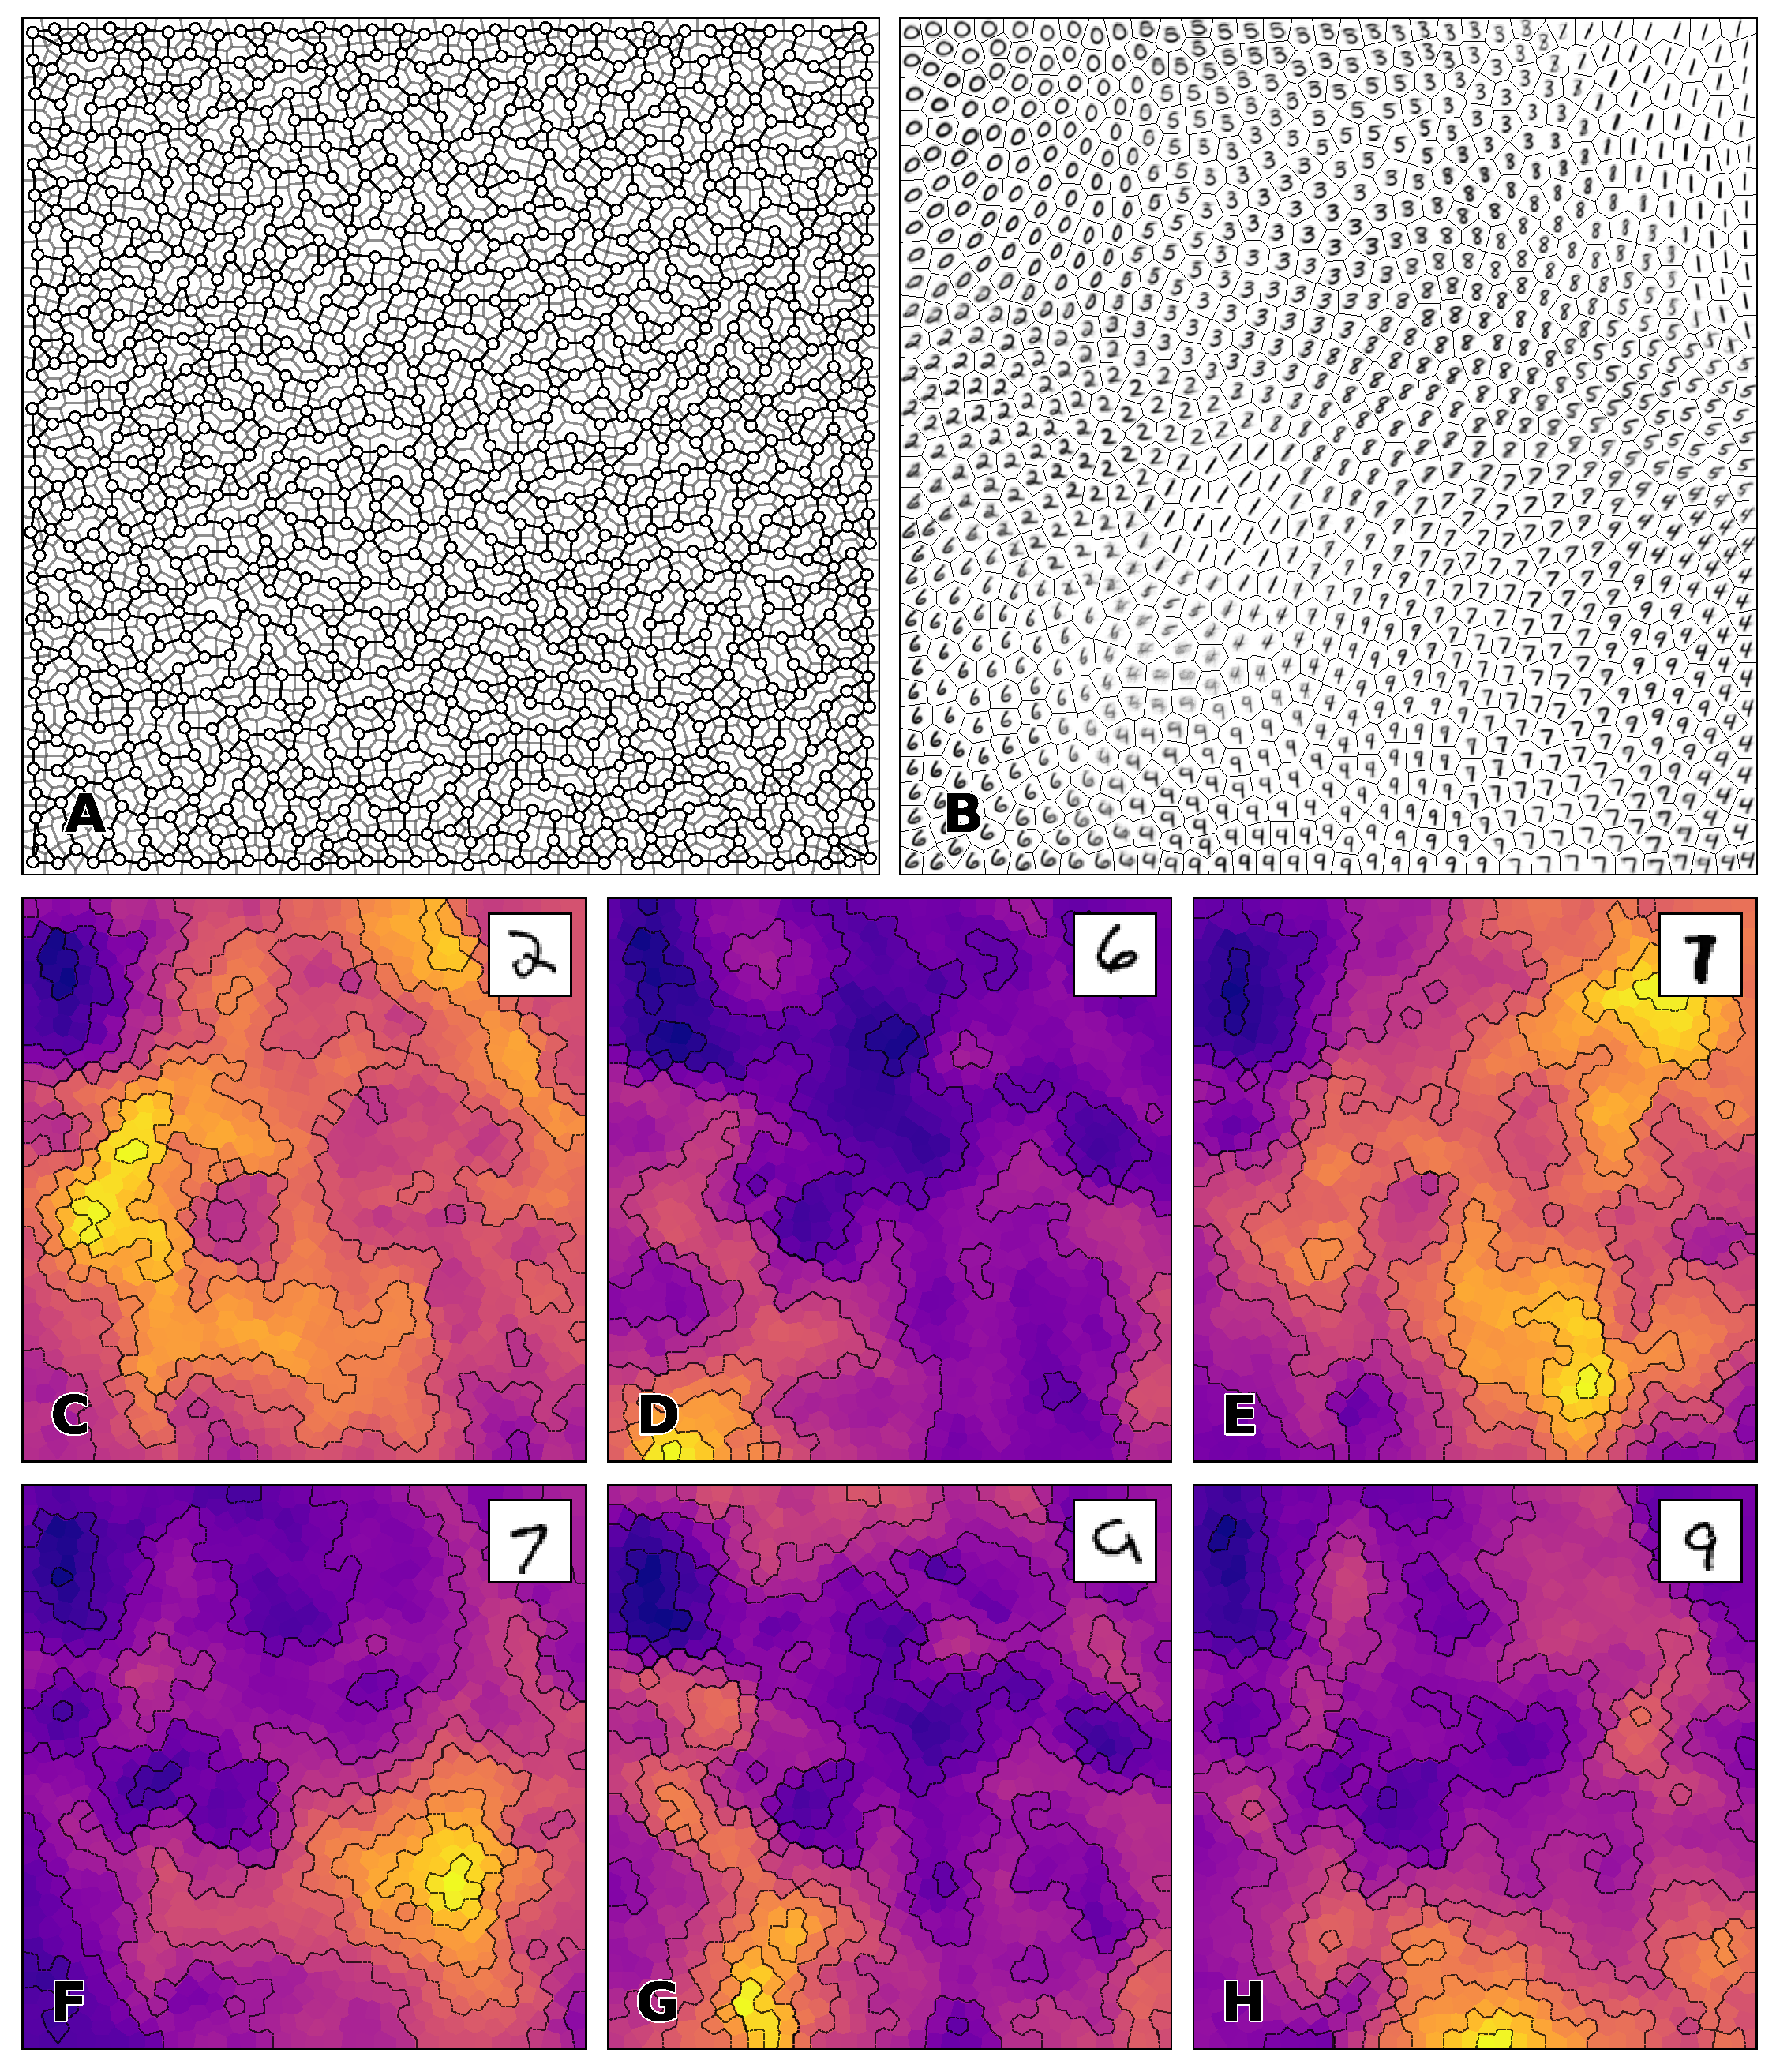
\includegraphics[width=\columnwidth]{experiment-MNIST.pdf}
  \vspace{2mm}
  \centering
  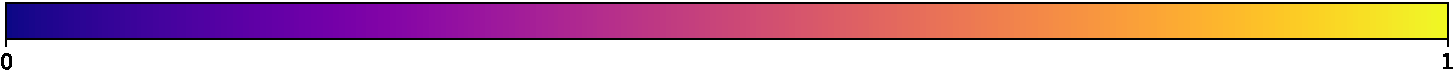
\includegraphics[width=.975\columnwidth]{figures/colormap.pdf}
  %
  \caption{%
  %
  {\bfseries \sffamily MNIST dataset (results)}
  %
  Randomized SOM made of $1024$ neurons with a $3$-nearest neighbors induced topology. Model has been trained for $25,000$ epochs on the MNIST dataset. \textbf{A} Map topology in neural space. \textbf{B} Map topology in data space. \textbf{C to H} Normalized distance map for six samples. Normalization has been performed for each sample in order to enhance contrast but this prevents comparison between maps.
  %
  }
  \label{fig:MNIST:results}
\end{figure}


\begin{figure}
  \centering
  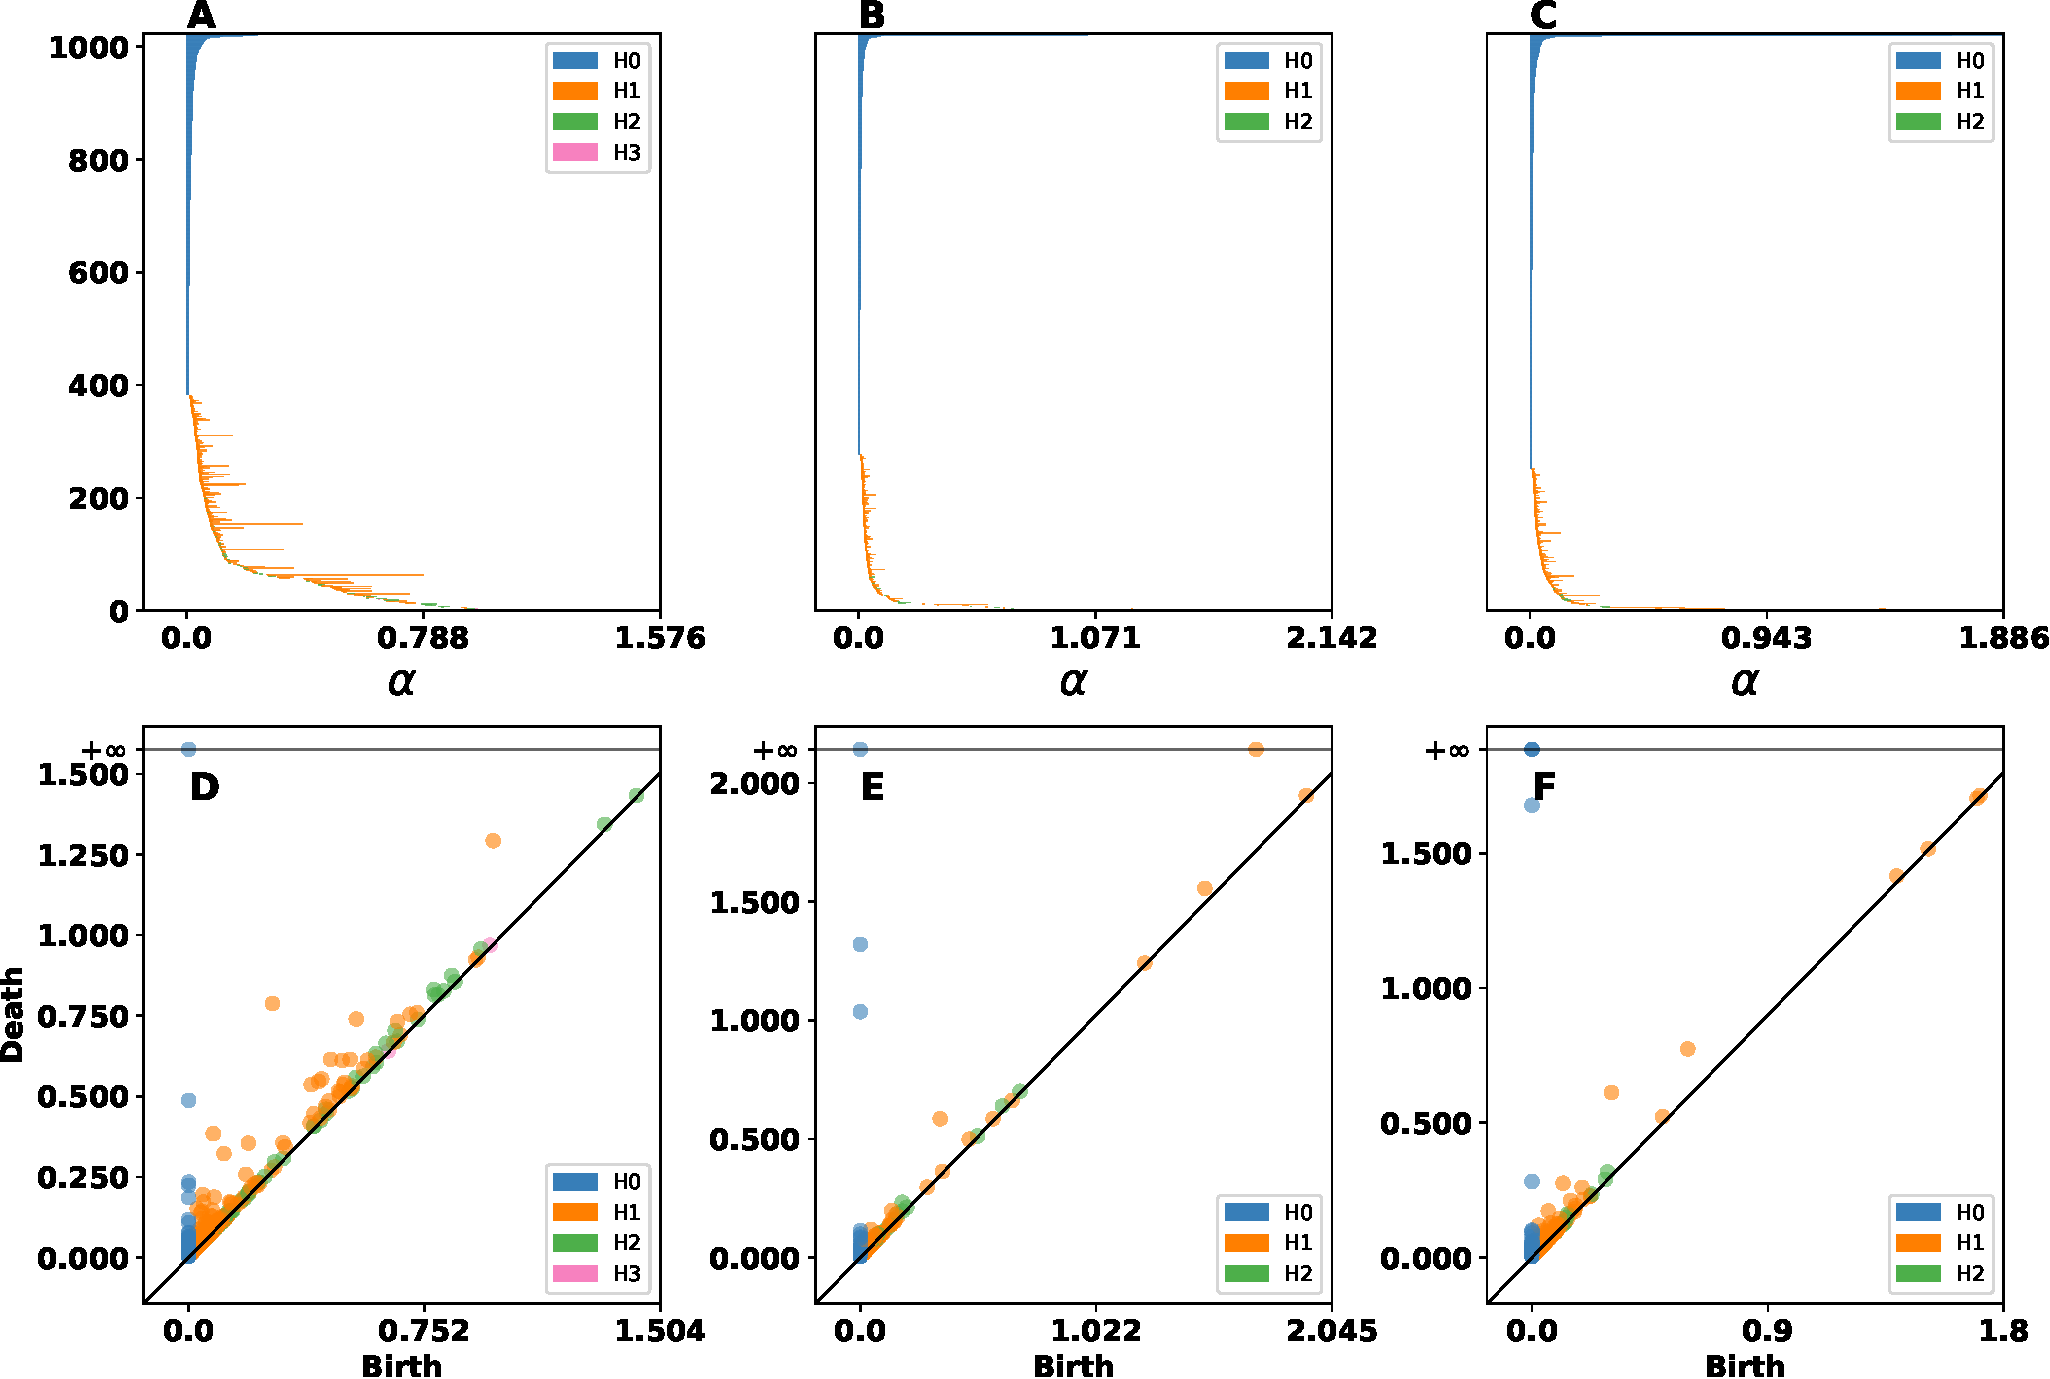
\includegraphics[width=\textwidth]{experiment-MNIST-analysis.pdf}
  \caption{{\bfseries \sffamily MNIST dataset (analysis)}
  Persistent Barcodes of \textbf{A} input space, \textbf{B} SOM, and \textbf{RSOM}.
  The blue, orange, and green line segments represent the $H0$-, $H1$-, and $H2$-homology,
  respectively. This means
  that blue color represents connected segments within the space, orange color reflects the holes
  within the space and green the voids. The longer the line segment the more important the 
  corresponding topological feature. \textbf{D} illustrates the persistent diagram for the input space.
  \textbf{E} and \textbf{F} depict the persistent diagrams for SOM and RSOM, respectively. Again blue dots
  indicate $H0$-homology features, orange dots represent $H1$-homolocical features, and green the 
  $H2$-homological features.}
  \label{fig:MNIST:analysis}
\end{figure}
\subsection{Reorganization following removal or addition of neurons}

The final and most challenging experiment is to test how the RSOM can cope
with degenerative cases, where either neurons die out (removal) or new units are added to the map (addition). Figure~\ref{fig:reorganization:results}A illustrates an example of a well-formed neural space (black outlined discs), a removal (red disks) and an addition (black dots). For both removal and addition, we applied a LLoyd relaxation scheme to achieve a new quasi-centroidal Voronoi tesselation. Figures \ref{fig:reorganization:results}B and \ref{fig:reorganization:results}C depicts the Voronoi tesselations after $100$ iterations starting from the initial tesselation shown in panel \ref{fig:reorganization:results}A. 

In order to conserve as much as possible the original topology, we used a differentiated procedure depending on if we are dealing with a removal or an addition. In case of removal, only the remaining neurons that were previously connected to a removed unit are allowed to connect to a new unit unconditionally. For the rest of the units, they might reconnect to a nearby unit if this unit is much closer than its closest current neighbour (85\% of the smallest distance to its current neighbours). In case of addition, new units can connect unconditionally to the nearest neighbours while old unit can only connect to the newly added unit if this unit is much closer than its current closest neighbour (85\% of the smallest distance to its current neighbours). This procedure guarantees that the topology is approximately conserved as shown in figures \ref{fig:reorganization:results}D-F. We tested the alternative of recomputing the graph from scratch but the resulting topology is quite different from the original because of micro-displacements of every units following the Lloyd relaxation.

Learning is performed in two steps. First we iterate $25,000$ epochs using the intact map, then we perform removal and addition and learning is iterated for another $5,000$ epochs for all three maps (orginal map, map with added units and map with removed units). The final self-organization is shown in figures \ref{fig:reorganization:results}G-I where we can observe strong similarities in the organization. For example, the central red patch is conserved in all three maps and the overall structure is visually similar. Of course, these results depend on the number of removed or added units (that needs to be relatively small compared to the size of the whole map) and their spatial distribution.
%\gid{the last two paragraphs are not too clear, they seem confusing}

%\gid{TODO Add a few more words here. Maybe make a connection to neuroscience facts about reorganization.} \npr{maybe in the discussion instead} \gid{Agreed} \nrp{Done}.

%Previous studies have shown that after an ablation or addition of units the map undergoes a reorganization of its neural representations. The immediate  consequence of a reorganization is the acquisition of new receptive fields. When an ablation takes place, unaffected neurons try to recover representations that got lost due to neurons death. In addition, on the other hand, the surplus neurons have to get their share of the representations and thus the entire map undergoes a reorganization.

%The induced topology shares similarity with the original topology (before ablation or addition). 

% It is known that this sort of reorganization takes place naturally within brain. More precisely, neurogenesis happens in the subgranular zone of the Dentate Gyrus (DG) of the hippocampus and in the subventricular zone of the lateral ventricle~\cite{Alvarez:2004}. On the other hand, when neural tissue in the cerebral cortex~\cite{Merzenich:1984,Taub:2014} or the spinal cord~\cite{Bareyre:2004,Liu:1958}, the undamaged neurons reorganize their receptive fields and undamaged nerves sprout new connections, respectively, partially or fully restore functionality. Therefore, the study of reorganization after a neural ablation or neurogenesis within a self-organizing map is detrimental. 


\begin{figure}
  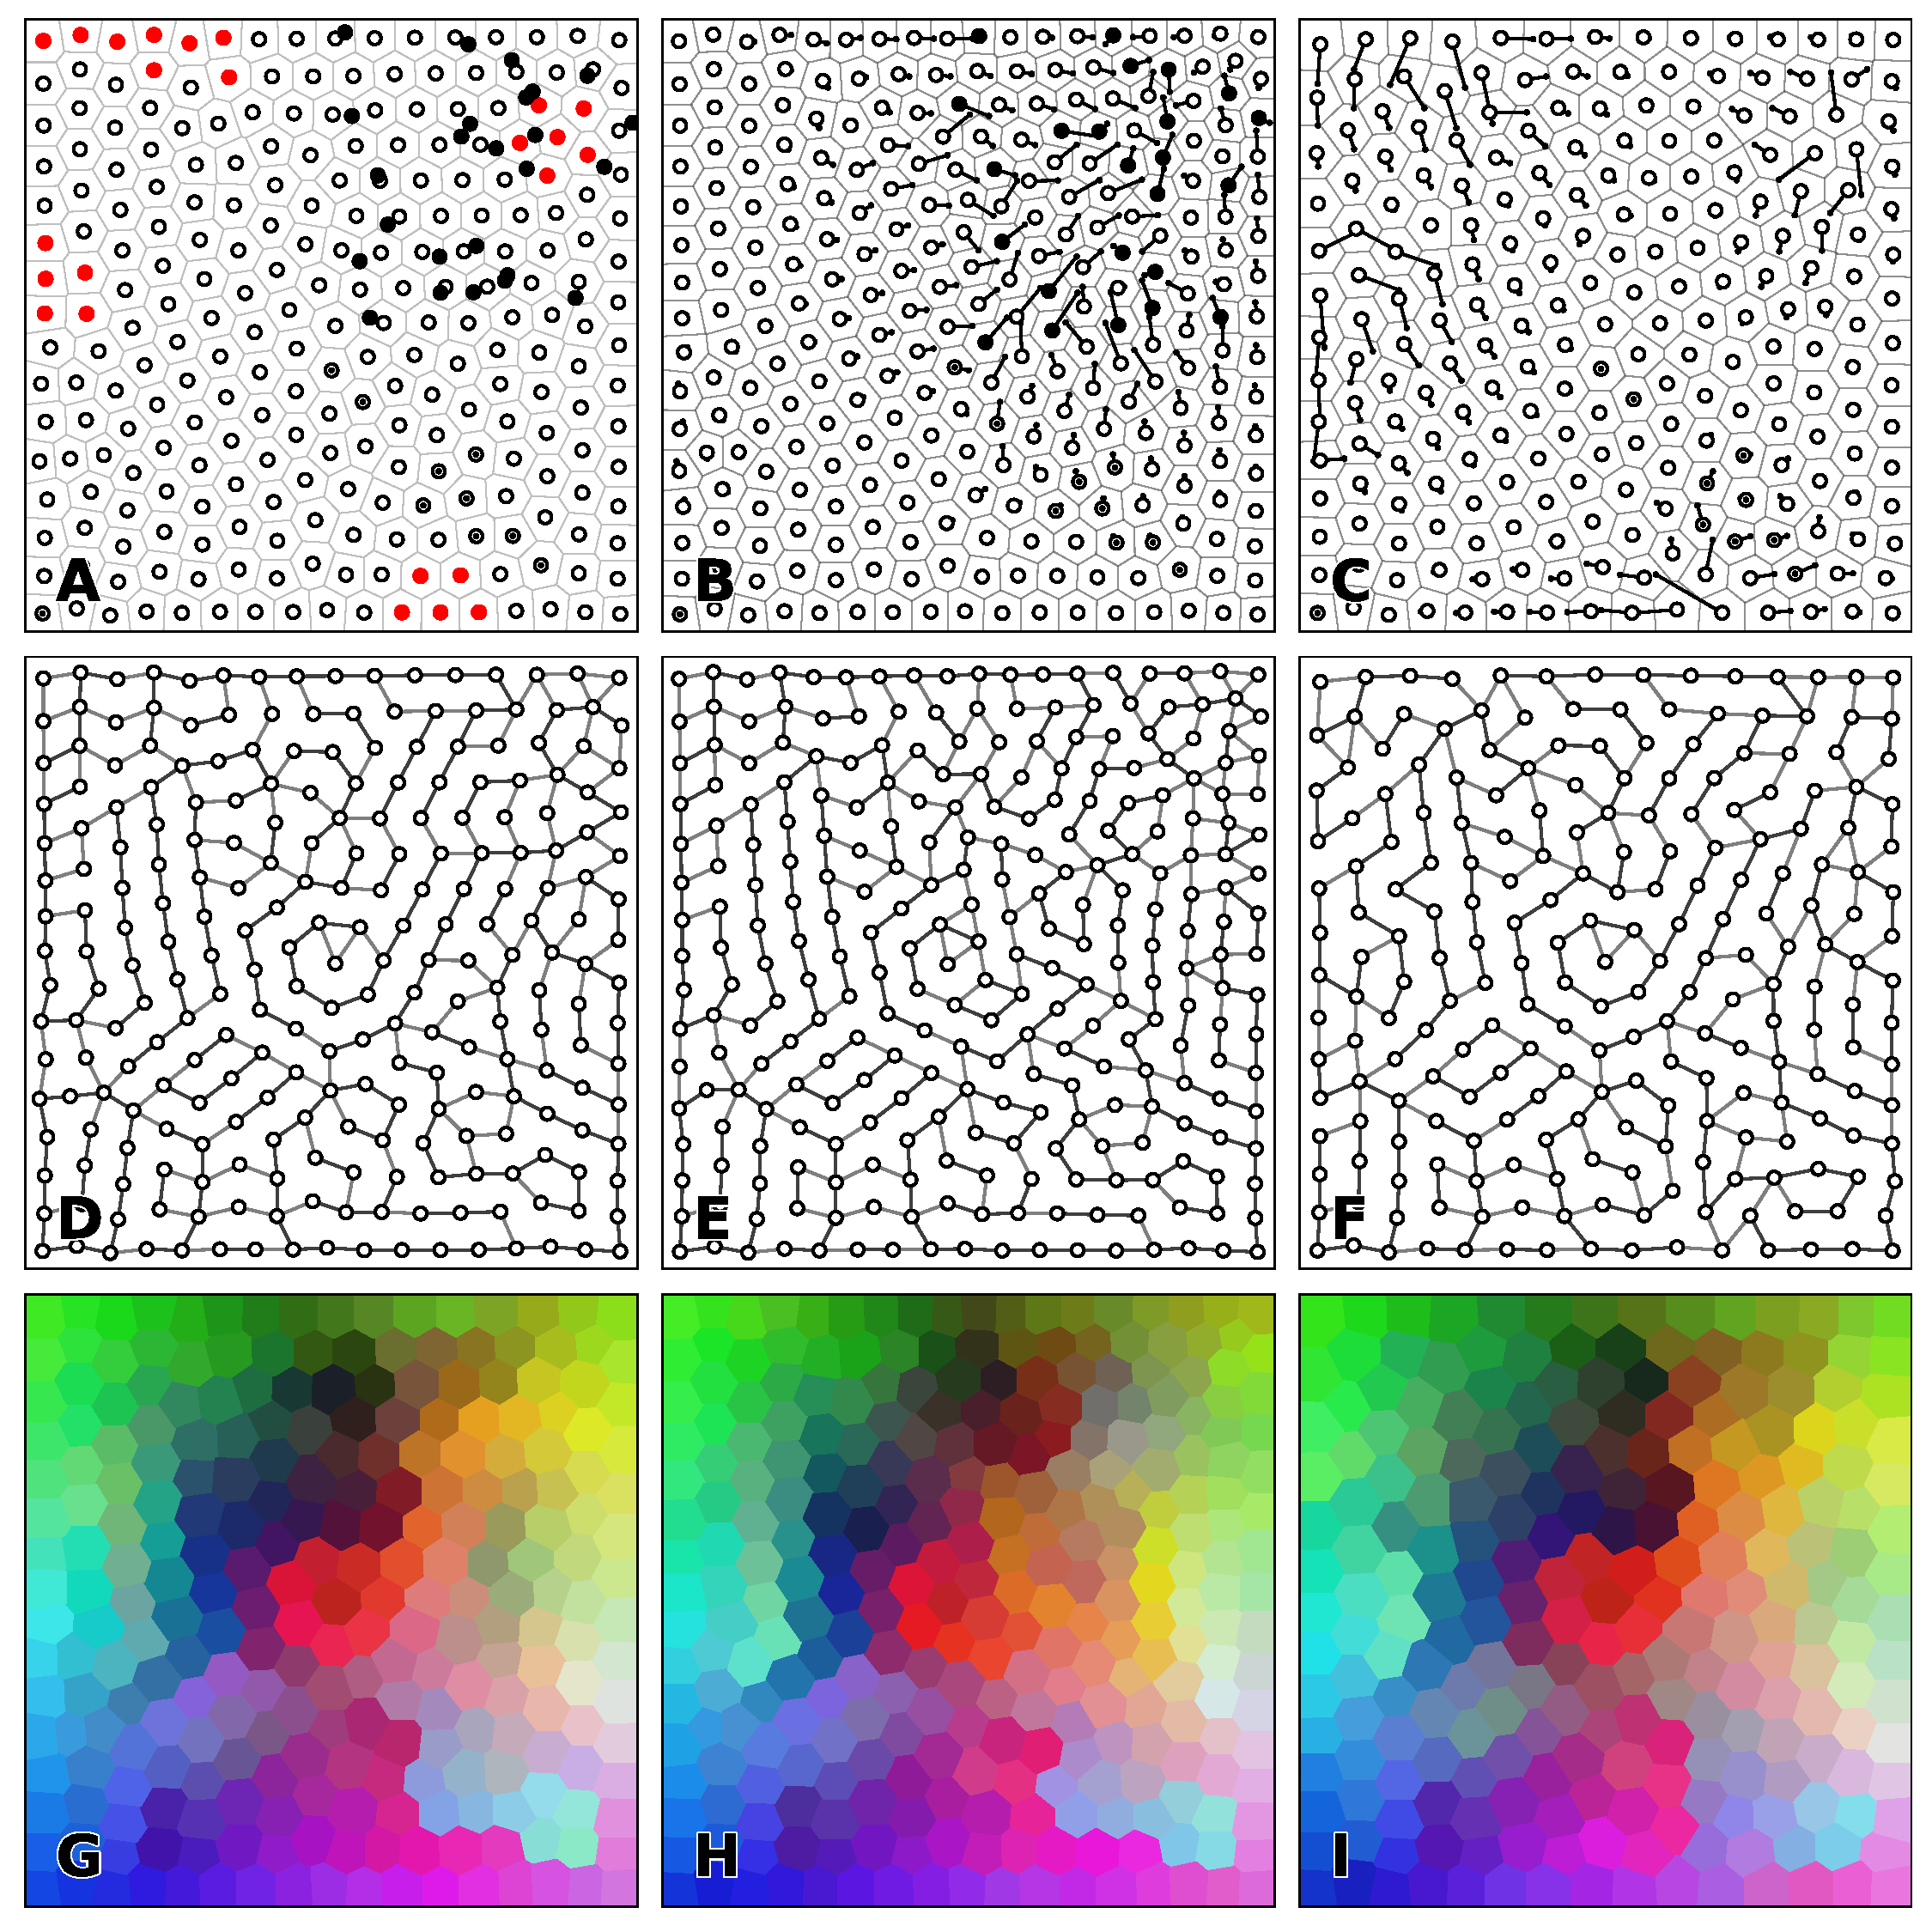
\includegraphics[width=\columnwidth]{experiment-reorganization.pdf}
  \caption{%
  {\bfseries \sffamily Reorganization (results).}
  %
  An initial set of 248 neurons (outlined discs on panel \textbf{A}) has been modified with the addition of 25 neurons (black discs) or the removal of 25 neurons (red discs). Panels \textbf{B} and \textbf{C} show the final position of neurons after 100 iterations of the centroidal Voronoi tesselation. Lines shows individual movement of neurons. Panels \textbf{D}, \textbf{E} and \textbf{F} show the 2-neighbors induced topology for \textbf{A}, \textbf{B} and \textbf{C} respectively. Panels \textbf{G}, \textbf{H} and \textbf{I} show the map
  map codebook for each map in neural space after learnin. Each voronoi cell of a neuron is painted with the color of the related codeword.
  %
  }
  \label{fig:reorganization:results}
\end{figure}



%We conduct five distinct experiments to investigate the proposed algorithm, VSOM, and its properties. Furthermore, for each experiment we train a Kohonen map to identify any potential difference with the VSOM.  The first experiment tests the ability of a two-dimensional map to learn representations of one-dimensional data. The second experiment consists of  two parts: in the first part the SOM algorithms learn to map a two-dimensional uniform distribution of an annulus on a two-dimensional neural space, and  in the second part they learn a two-dimensional Euclidean plane with holes. Three-dimensional points uniformly distributed on a cube are being mapped by the two SOM algorithms on two-dimensional neural space in the third experiment. In the fourth experiment, we tested how VSOM and Kohonen can map the MNIST hand-written digits on a two-dimensional neural space.  Finally, we investigate how the neural space is being reorganized after a removal of some of the neural units (ablation) or after the injection of new neural units in the map (neurogenesis). It is known that this sort of reorganization takes place naturally within brain. More precisely, neurogenesis happens in the subgranular zone of the Dentate Gyrus (DG) of the hippocampus and in the subventricular zone of the lateral ventricle~\cite{Alvarez:2004}. On the other hand, when neural tissue in the cerebral cortex~\cite{Merzenich:1984,Taub:2014} or the spinal cord~\cite{Bareyre:2004,Liu:1958}, the undamaged neurons reorganize their receptive fields and undamaged nerves  sprout new connections, respectively, partially or fully restore functionality. Therefore, the study of reorganization after a neural ablation or neurogenesis within a self-organizing map is detrimental. 

% In the following sections we provide results regarding the VSOM in main figures. However, we have run experiments using both the Kohonen and the VSOM learning algorithms (except the reorganization case, where we use only the VSOM algorithm). When we analyze the results using the eigenvalues distribution method or the persistence diagrams we present results for both the VSOM and the Kohonen. Furthermore, we provide figures regarding the cases of: (i) the two-dimensional data set with random holes on a plain, (ii) a three dimensional uniform distribution, and (iii) the MNIST hand written digits set in the main text. The rest of the results are given in the Supplementary Material. 

%\begin{table}[!ht]
%  \begin{center}
%    \begin{tabular}{ccccc}
%        \textbf{Algorithm} & $d_b$ $H0$ & $W_p$ $(H0)$ & $d_b$ $H1$ & $W_p$ $(H1)$ \\
%        \hline
%        Kohonen & 0.0811 & 0.0549 & 15.1644 & 9.2962 \\
%        VSOM    & 0.0811 & 0.0450 & 21.6092 & 7.4033
%      \end{tabular}
%      \caption{\textbf{Experiment $3$ Persistence Diagram Distances.} Bottleneck      and Wasserstein distances between the persistence diagrams of the input and Kohonen and VSOM. In this experiment both the Kohonen and the VSOM do not express any significant difference. $d_b$ is the bottleneck distance~\eqref{eq:bottle}, $W_p$ is the Wasserstein distance~\eqref{eq:wasser}, $H0$ indicates the Homology Group $0$ (path-connected components, or one-dimensional holes), $H1$ is the Hologoy group $1$ (two-dimensional holes).}
      %\label{table:parameters}
%  \end{center}
% \end{table}


